\documentclass[a4paper,12pt]{article}

% -----------------------------------------------------------------------------
% Packages and page setup
% -----------------------------------------------------------------------------
\usepackage[utf8]{inputenc}
\usepackage[T1]{fontenc}
\usepackage{lmodern}
\usepackage{microtype}
\usepackage[a4paper,margin=1in]{geometry}
\usepackage{setspace}
\usepackage{graphicx}
\usepackage{float}
\usepackage{amsmath,amssymb}
\usepackage{booktabs}
\usepackage{tabularx}
\usepackage{array}
\usepackage{makecell}
\usepackage{siunitx}
\usepackage{xcolor}
\usepackage{xurl}
\usepackage{enumitem}
\usepackage{listings}
\usepackage{caption}
\usepackage{subcaption}
\usepackage{tikz}
\usetikzlibrary{arrows.meta,positioning,fit,calc,shapes.geometric}
\usepackage[most]{tcolorbox}
\usepackage{fancyhdr}
\usepackage{hyperref}

\setstretch{1.08}
\setlength{\parindent}{0pt}
\setlength{\parskip}{0.55em}
\setlength{\emergencystretch}{3em}
\setlength{\headheight}{14.5pt}
\setlist[itemize]{topsep=0.35em,itemsep=0.2em,parsep=0pt,leftmargin=1.6em}
\setlist[enumerate]{topsep=0.35em,itemsep=0.25em,parsep=0pt,leftmargin=1.8em}
\captionsetup{font=small,labelfont=bf}
\sisetup{detect-all}

% -----------------------------------------------------------------------------
% Colours and reusable styles
% -----------------------------------------------------------------------------
\definecolor{uaGreen}{HTML}{8FD400}
\definecolor{navy}{HTML}{172033}
\definecolor{softBlue}{HTML}{EAF3FF}
\definecolor{softOrange}{HTML}{FFF2E3}
\definecolor{softGreen}{HTML}{E8FAF5}
\definecolor{softPurple}{HTML}{F2EDFF}
\definecolor{softRed}{HTML}{FFF0F0}
\definecolor{lineGray}{HTML}{5B6B82}
\definecolor{lightGray}{HTML}{F4F6F9}

\newcolumntype{Y}{>{\raggedright\arraybackslash}X}
\newcolumntype{C}[1]{>{\centering\arraybackslash}p{#1}}
\newcolumntype{L}[1]{>{\raggedright\arraybackslash}p{#1}}

\newtcolorbox{keypoint}[1][]{
    enhanced,
    colback=softBlue,
    colframe=navy!65,
    boxrule=0.8pt,
    arc=2mm,
    left=3mm,right=3mm,top=2mm,bottom=2mm,
    title=#1,
    fonttitle=\bfseries
}

\newtcblisting{terminalbox}[1]{
    enhanced,
    breakable,
    colback=black!2,
    colframe=black!55,
    boxrule=0.7pt,
    arc=1.5mm,
    title={#1},
    fonttitle=\bfseries,
    listing only,
    listing options={
        basicstyle=\ttfamily\small,
        breaklines=true,
        columns=fullflexible,
        showstringspaces=false,
        keepspaces=true,
        language={}
    }
}

\lstdefinestyle{pseudocode}{
    basicstyle=\ttfamily\small,
    frame=single,
    rulecolor=\color{black!35},
    backgroundcolor=\color{black!2},
    breaklines=true,
    columns=fullflexible,
    showstringspaces=false,
    xleftmargin=0.5em,
    xrightmargin=0.5em
}

\hypersetup{
    colorlinks=true,
    linkcolor=navy,
    citecolor=navy,
    urlcolor=blue!65!black,
    pdftitle={Mind the Gap: Autonomous V2X Lane Merging},
    pdfauthor={André Alexandre and Bernardo Marujo},
    pdfpagemode=UseOutlines
}

\pagestyle{fancy}
\fancyhf{}
\fancyhead[L]{\small Mind the Gap}
\fancyhead[R]{\small Redes e Sistemas Autónomos}
\fancyfoot[C]{\thepage}
\renewcommand{\headrulewidth}{0.4pt}

\newcommand{\repositoryURL}{https://github.com/BMarujo/RSA}

\begin{document}
\pagenumbering{gobble}

% -----------------------------------------------------------------------------
% Title page
% -----------------------------------------------------------------------------
\begin{titlepage}
    \centering
    \vspace*{1.4cm}

    {\Large \textbf{Redes e Sistemas Autónomos}}\\[0.8cm]
    {\Huge \textbf{Mind the Gap}}\\[0.25cm]
    {\LARGE Autonomous V2X Lane Merging}\\[0.65cm]
    {\large Project Report}\\[1.3cm]

    \rule{0.82\textwidth}{0.8pt}\\[1.0cm]

    \begin{tabular}{c}
        {\Large André Alexandre -- 114143 -- 50\%}\\[0.25cm]
        {\Large Bernardo Marujo -- 107322 -- 50\%}
    \end{tabular}

    \vspace{0.8cm}
    \textbf{alexandreandre@ua.pt}\\
    \textbf{bernardomarujo@ua.pt}\\[0.6cm]

    \href{\repositoryURL}{\textbf{GitHub repository: BMarujo/RSA}}\\[0.3cm]
    % TODO before submission: replace the line below with the public video URL
    % or with the permalink to the message posted in the course Discord channel.
    \textit{Demo video: insert the public URL or Discord message link before submission.}

    \vfill

    \includegraphics[width=0.18\textwidth]{ua.png}\\[0.45cm]
    {\large University of Aveiro}\\
    {\large Department of Electronics, Telecommunications and Informatics}\\
    {\large Academic Year 2025/2026}
\end{titlepage}

\pagenumbering{roman}

\begin{abstract}
This report presents a software-in-the-loop prototype for decentralized V2X lane merging. Each simulated vehicle is represented by an independent On-Board Unit (OBU) that combines local sensor data with Cooperative Awareness Messages (CAMs) and Maneuver Coordination Messages (MCMs). The OBU estimates time of arrival to a fixed merge point, identifies a lead vehicle and a cooperative host, negotiates a temporal gap, checks safety conditions, and publishes speed and lane commands. SUMO provides the road and vehicle dynamics, while a Python TraCI bridge translates MQTT actuator messages into physical simulation actions and returns execution feedback. The implementation separates logical authorization from physical lane-change execution through the states \texttt{WAIT\_EDGE}, \texttt{APPLY}, and \texttt{CLEAR}. A representative \texttt{single-lane} demonstration shows host rejection and reselection, successful MCM acceptance, delayed lane availability, physical merge execution, rear-gap protection, and a clean completion.
\end{abstract}

\tableofcontents
\newpage
\pagenumbering{arabic}

% -----------------------------------------------------------------------------
% 1. Introduction
% -----------------------------------------------------------------------------
\section{Introduction}

Lane merging is a short maneuver with a high coordination requirement. A vehicle entering from an access ramp must identify a suitable gap, adapt its speed, and avoid forcing a main-lane vehicle into an unsafe reaction. When traffic is dense, a purely individual decision based only on the merge vehicle's local perception can be insufficient: the intended follower may need to slow down and preserve the selected gap.

\textit{Mind the Gap} addresses this problem with a decentralized V2X prototype. The system combines SUMO, TraCI, MQTT, Vanetza, and Docker. Each vehicle runs an independent OBU application that receives its own simulated sensor state, learns the kinematic state of nearby vehicles through CAMs, and uses MCMs to request, accept, or reject a cooperative maneuver. SUMO does not choose the merge slot or authorize cooperation; it simulates the road and executes commands produced by the OBUs.

A central design principle is the separation between \emph{logical coordination} and \emph{physical execution}. An MCM acceptance indicates that a host is willing to cooperate, but the merge is not considered physically active until the target lane exists and the TraCI bridge can apply the lane command. This distinction is especially visible in the \texttt{single-lane} scenario used in the demonstration, where the ramp edge initially contains only lane index 0 while the requested target lane is lane index 1 on a later edge.

\subsection{Objectives of the Work}

The main objective is to design and demonstrate a reproducible software-in-the-loop system in which vehicles coordinate a lane merge through local OBU decisions and V2X message exchange. The work focuses on four concrete goals:

\begin{itemize}
    \item implement one independent, containerized OBU per SUMO vehicle;
    \item derive local awareness from CAMs and negotiate cooperation through MCMs;
    \item compute a safe temporal merge slot and enforce safety guards before and during execution;
    \item validate the end-to-end flow in the \texttt{single-lane} scenario, from sensor publication to merge completion.
\end{itemize}

The resulting prototype answers an engineering question rather than attempting a complete production deployment: can a ramp vehicle select and execute a cooperative merge while the decision logic remains outside SUMO and distributed across the participating OBUs?

\subsection{Scope and Contributions}

The contribution is an integrated architecture and implementation rather than a new communication standard. The project provides: a Docker-based SITL stack; a per-vehicle OBU model; CAM-based neighbor tracking; MCM request/accept/reject handling; ETA-based role and slot selection; a five-state merge FSM; host reservation and yielding; final, TTC, car-following, and rear-gap guards; and a TraCI execution protocol with explicit lane-command feedback.

The report concentrates on the current code in the repository. Documentation files were used as context, but behavior described here was checked against the implementation modules and the stored \texttt{single-lane} run log.

% -----------------------------------------------------------------------------
% 2. Architecture
% -----------------------------------------------------------------------------
\section{System Architecture}

Figure~\ref{fig:architecture} shows the complete software-in-the-loop architecture. Two communication paths are deliberately separated. Sensor, actuator, and status information is exchanged through MQTT, whereas CAM and MCM packets are encoded by Vanetza and exchanged through simulated UDP broadcast over the Docker network.

\begin{figure}[H]
    \centering
    \includegraphics[width=\linewidth]{RSA.drawio.png}
    \caption{Overall architecture of the decentralized V2X lane-merging system.}
    \label{fig:architecture}
\end{figure}

\subsection{Simulation and Control Path}

SUMO is the physical simulation engine. It owns the road graph, edges, lanes, vehicle positions, speeds, and motion. A Python TraCI bridge advances the simulation, reads each vehicle state, and publishes a compact sensor payload containing position, speed, heading, lane identifier, and simulation time. The bridge also subscribes to actuator topics and applies speed, speed-mode, and lane commands to SUMO.

The shared MQTT broker decouples the bridge from the OBUs. For a vehicle with identifier \texttt{Merge\_Car}, the main closed-loop path is:

\begin{center}
\small
\path{car/Merge_Car/sensors/gps}
$\rightarrow$ OBU decision
$\rightarrow$ \path{car/Merge_Car/actuators/...}
$\rightarrow$ TraCI/SUMO.
\end{center}

The bridge returns lane execution state on \path{car/Merge_Car/status/lane_command}. Consequently, the OBU can distinguish between issuing a command and observing that SUMO has actually executed it.

\begin{keypoint}[Responsibility boundary]
The OBU selects the slot, negotiates the maneuver, checks safety, and produces targets. The TraCI bridge translates targets into API calls. SUMO simulates the resulting motion. Neither the bridge nor SUMO chooses which vehicle should cooperate.
\end{keypoint}

\subsection{Per-Vehicle OBU Container}

The scenario generator creates one OBU service for every explicit vehicle in the SUMO route file. Each container contains three cooperating processes:

\begin{itemize}
    \item a Python OBU application implementing the FSM and calculations;
    \item an embedded Mosquitto broker acting as the vehicle's local message bus;
    \item Vanetza \texttt{socktap}, which encodes and decodes C-ITS messages.
\end{itemize}

The local broker bridges only selected topics to the shared broker. It imports the vehicle's own sensors and lane-command status, imports peer FSM summaries, and exports that vehicle's actuator and FSM status topics. Raw kinematics of other vehicles are not imported from SUMO; they are primarily reconstructed from CAMs. Peer FSM summaries are used for coordination metadata such as whether a candidate host already has an active reservation.

\subsection{V2X Communication Path}

The OBU publishes JSON templates to \path{vanetza/in/cam}, \path{vanetza/in/mcm}, or \path{vanetza/in/denm}. Vanetza serializes the message and broadcasts it on the simulated radio interface. Other OBU containers decode the packet and publish the resulting JSON on the corresponding \path{vanetza/out/...} topic. CAM and MCM traffic therefore follows a different path from the simulator's sensor and actuator traffic.

CAMs are periodic awareness messages. MCMs are event-driven cooperation messages. DENM support is present, but it is disabled by default and is not part of the merge decision demonstrated in this report.

\subsection{Main MQTT Interfaces}

Table~\ref{tab:mqtt} summarizes the interfaces that cross the boundary between the shared broker, the bridge, and the local OBU brokers. A \texttt{tabularx} layout is used to keep long topics within the page margins.

\begin{table}[H]
\centering
\small
\caption{Main MQTT interfaces.}
\label{tab:mqtt}
\begin{tabularx}{\linewidth}{L{0.38\linewidth} L{0.17\linewidth} Y}
\toprule
\textbf{Topic} & \textbf{Publisher} & \textbf{Purpose} \\
\midrule
\path{car/<id>/sensors/gps} & TraCI bridge & Position, speed, heading, lane ID, and simulation time for the local vehicle. \\
\path{car/<id>/actuators/speed} & OBU & Desired longitudinal speed. \\
\path{car/<id>/actuators/lane} & OBU & Desired SUMO lane index. \\
\path{car/<id>/actuators/speed_mode} & OBU & SUMO speed-control mode used while applying the target. \\
\path{car/<id>/status/fsm} & OBU & Role, FSM state, ETA, command targets, reservation metadata, and completion counters. \\
\path{car/<id>/status/lane_command} & TraCI bridge & Execution feedback: \texttt{WAIT\_EDGE}, \texttt{APPLY}, \texttt{CLEAR}, or \texttt{FAILED}. \\
\bottomrule
\end{tabularx}
\end{table}

\subsection{Dynamic Deployment}

\path{scripts/run_vanetza_scenario.sh} selects a scenario, establishes scenario-specific environment defaults, invokes \path{scripts/generate_obu_compose.py}, and starts Docker Compose. The generator parses the referenced SUMO route files, extracts explicit vehicle identifiers, assigns station IDs and MAC addresses, classifies ramp and main-lane vehicles, and writes a generated Compose override. This mechanism avoids maintaining a static service definition for every vehicle and guarantees that the bridge and OBU set are derived from the same scenario.

% -----------------------------------------------------------------------------
% 3. Implementation
% -----------------------------------------------------------------------------
\section{Implementation}

\subsection{Code Organization and Periodic Control Loop}

The OBU implementation is split into focused modules rather than a single monolithic controller. Table~\ref{tab:modules} lists the main groups.

\begin{table}[H]
\centering
\small
\caption{Main implementation modules.}
\label{tab:modules}
\begin{tabularx}{\linewidth}{L{0.32\linewidth} Y}
\toprule
\textbf{Path or module} & \textbf{Responsibility} \\
\midrule
\path{obu/app/main.py}, \path{config.py} & OBU construction, MQTT subscriptions, state variables, environment-based configuration, and helper methods. \\
\path{messaging.py}, \path{vanetza_codec.py}, \path{geometry.py} & CAM/MCM construction and parsing, coordinate conversion, lane parsing, actuator publication, and status publication. \\
\path{fsm_core.py}, \path{fsm_merge_role.py}, \path{fsm_merge_negotiation.py} & Periodic decision loop, merge-vehicle behavior, request/retry/response matching, authorization, and commitment. \\
\path{fsm_host.py}, \path{car_following.py}, \path{fsm_merge_guards.py}, \path{merge_support.py} & Host reservation, lead behavior, following control, slot selection, safety guards, completion logic, and diagnostics. \\
\path{sim/bridge/traci_bridge.py} & Sensor publication, actuator application, lane-command feedback, collision guard, and SUMO-GUI overlays. \\
\bottomrule
\end{tabularx}
\end{table}

The OBU's \texttt{step()} method schedules four activities independently. With the scenario defaults, CAM publication, FSM execution, and actuator publication occur every \SI{100}{ms}, while status is published every \SI{250}{ms}. At every FSM step, stale neighbors and MCMs are pruned, the effective role is recomputed, a base speed target is selected, the role-specific FSM runs, and CAM-based car-following is applied last.

\subsection{Single-Lane Scenario}

The demonstration contains four main-lane vehicles and one ramp vehicle. Because station IDs are assigned in route-file order, the current mapping is shown in Table~\ref{tab:stations}.

\begin{table}[H]
\centering
\small
\caption{Vehicle and station mapping used in the representative \texttt{single-lane} run.}
\label{tab:stations}
\begin{tabularx}{0.9\linewidth}{C{0.16\linewidth} L{0.30\linewidth} Y}
\toprule
\textbf{Station} & \textbf{Vehicle} & \textbf{Function in the demonstration} \\
\midrule
101 & \texttt{Main\_Lead} & Main-lane traffic ahead of the selected slot. \\
102 & \texttt{Main\_Front} & Main-lane vehicle that can become the current lead. \\
103 & \texttt{Main\_Acceptor} & Candidate host; rejects when the available ETA gap becomes too small. \\
104 & \texttt{Main\_Back} & Cooperative host selected for the successful maneuver. \\
105 & \texttt{Merge\_Car} & Ramp vehicle requesting and executing the merge. \\
\bottomrule
\end{tabularx}
\end{table}

The Aveiro configuration uses merge point $(194.89, 2212.42)$ in SUMO coordinates, ramp edge \texttt{34126779}, and target lane index 1. The \texttt{single-lane} launcher sets an MCM request distance of \SI{80}{m}, a nominal cruise speed of \SI{7.5}{m/s}, safe and commit headways of \SI{1.5}{s}, a lane-change duration of \SI{2}{s}, a host reservation of \SI{5}{s}, and a maximum reservation lifetime of \SI{14}{s}.

Figure~\ref{fig:scenario} presents the logical geometry. The roles are not permanently assigned: they are recomputed from the current ordering of ETAs and reservation state.

\begin{figure}[H]
\centering
\resizebox{0.96\linewidth}{!}{%
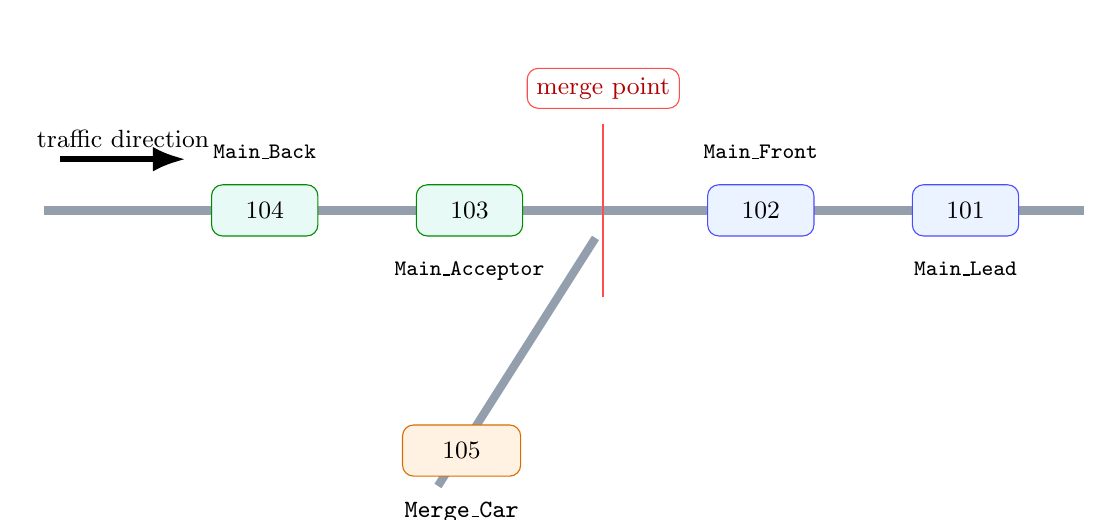
\begin{tikzpicture}[>=Latex, font=\small]
    \draw[line width=3pt, draw=lineGray!65] (0,2) -- (13.2,2);
    \draw[line width=3pt, draw=lineGray!65] (5.0,-1.5) -- (7.0,1.65);
    \draw[line width=2pt, ->] (0.2,2.65) -- (1.8,2.65) node[midway,above]{traffic direction};
    \draw[red!70, thick] (7.1,0.9) -- (7.1,3.1);
    \node[draw=red!70, rounded corners, fill=white, text=red!70!black] at (7.1,3.55) {merge point};

    \node[draw=blue!70, fill=softBlue, rounded corners, minimum width=1.35cm, minimum height=0.65cm] (v101) at (11.7,2) {101};
    \node[below=2mm of v101, font=\footnotesize] {\texttt{Main\_Lead}};
    \node[draw=blue!70, fill=softBlue, rounded corners, minimum width=1.35cm, minimum height=0.65cm] (v102) at (9.1,2) {102};
    \node[above=2mm of v102, font=\footnotesize] {\texttt{Main\_Front}};
    \node[draw=green!55!black, fill=softGreen, rounded corners, minimum width=1.35cm, minimum height=0.65cm] (v103) at (5.4,2) {103};
    \node[below=2mm of v103, font=\footnotesize] {\texttt{Main\_Acceptor}};
    \node[draw=green!55!black, fill=softGreen, rounded corners, minimum width=1.35cm, minimum height=0.65cm] (v104) at (2.8,2) {104};
    \node[above=2mm of v104, font=\footnotesize] {\texttt{Main\_Back}};
    \node[draw=orange!85!black, fill=softOrange, rounded corners, minimum width=1.5cm, minimum height=0.65cm] (v105) at (5.3,-1.05) {105};
    \node[below=2mm of v105] {\texttt{Merge\_Car}};
\end{tikzpicture}}
\caption{Logical arrangement of the five vehicles in the \texttt{single-lane} demonstration.}
\label{fig:scenario}
\end{figure}

\subsection{CAM-Based Neighbor Awareness}

The TraCI bridge publishes the local SUMO state, and the OBU converts it into a CAM. The position is converted from local $(x,y)$ coordinates to latitude and longitude using a local tangent approximation around the configured origin. On reception, the inverse conversion reconstructs SUMO-like coordinates. The OBU stores, for each station, position, speed, heading, distance to the merge point, distance change, and the simulation timestamp.

The distance of vehicle $i$ to the merge reference point is

\begin{equation}
    d_i = \sqrt{(x_i-x_m)^2 + (y_i-y_m)^2},
    \label{eq:distance}
\end{equation}

and its estimated time of arrival is

\begin{equation}
    \eta_i = \frac{d_i}{\max(v_i,0.1)}.
    \label{eq:eta}
\end{equation}

The lower bound of \SI{0.1}{m/s} prevents division by zero. Stale observations can be projected forward using the last speed and heading for a limited guard interval. This memory is used by the final guard so that a briefly missing CAM does not immediately erase a nearby vehicle.

\subsection{Role Resolution and Slot Selection}

A ramp vehicle is assigned the effective role \texttt{merge} until it completes the maneuver. Main-lane vehicles compare their ETA with the merge candidate. A vehicle that arrives earlier is a potential \texttt{lead}; one that arrives later is a potential \texttt{host}. An active reservation overrides this ordering and forces the corresponding main-lane OBU to continue as host.

The merge vehicle sorts main-lane candidates by ETA. The first candidate with $\eta_i \geq \eta_M$ becomes the host, while the previous candidate becomes the lead. A host whose shared FSM status reports an active reservation for another station is skipped. If no candidate exists after the merge vehicle, the algorithm identifies an \emph{after-last-main} situation and may use lead-only authorization, but only after all safety guards pass.

For lead ETA $\eta_L$ and host ETA $\eta_H$, the code constructs the safe temporal interval

\begin{align}
    \eta_{\min} &= \eta_L + h_{\mathrm{safe}}, \\
    \eta_{\max} &= \eta_H - h_{\mathrm{commit}},
    \label{eq:window}
\end{align}

where $h_{\mathrm{safe}}$ protects the gap behind the lead and $h_{\mathrm{commit}}$ protects the gap in front of the host. The desired ETA is the merge vehicle's current ETA clamped to this interval. A slot is feasible when $\eta_{\max} \geq \eta_{\min}$ whenever both bounds exist.

\begin{figure}[H]
\centering
\resizebox{0.94\linewidth}{!}{%
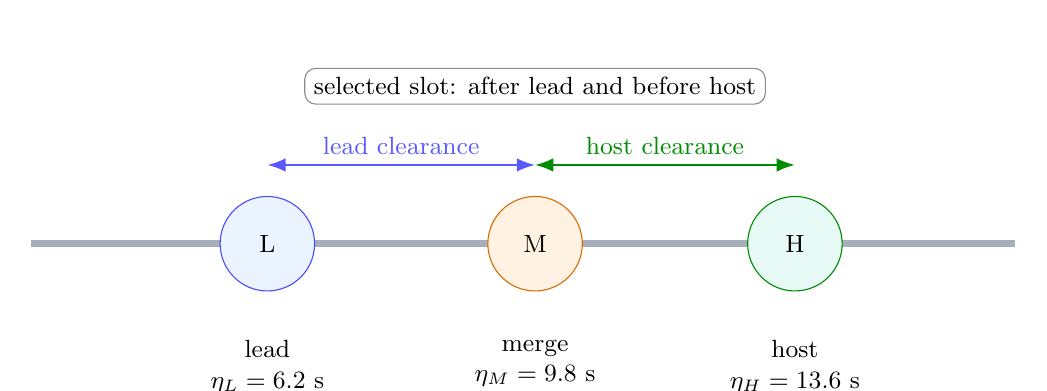
\begin{tikzpicture}[>=Latex, font=\small]
    \draw[line width=2.5pt, draw=lineGray!55] (0,0) -- (12.5,0);
    \node[circle, draw=blue!70, fill=softBlue, minimum size=12mm] (lead) at (3.0,0) {L};
    \node[circle, draw=orange!85!black, fill=softOrange, minimum size=12mm] (merge) at (6.4,0) {M};
    \node[circle, draw=green!55!black, fill=softGreen, minimum size=12mm] (host) at (9.7,0) {H};
    \node[below=5mm of lead, align=center] {lead\\$\eta_L=6.2$ s};
    \node[below=5mm of merge, align=center] {merge\\$\eta_M=9.8$ s};
    \node[below=5mm of host, align=center] {host\\$\eta_H=13.6$ s};
    \draw[<->, thick, blue!65] (3.0,1.0) -- (6.4,1.0) node[midway,above]{lead clearance};
    \draw[<->, thick, green!55!black] (6.4,1.0) -- (9.7,1.0) node[midway,above]{host clearance};
    \node[draw=black!45, rounded corners, fill=white, align=center] at (6.4,2.0) {selected slot: after lead and before host};
\end{tikzpicture}}
\caption{ETA ordering used to choose the lead, merge vehicle, and cooperative host.}
\label{fig:eta_slot}
\end{figure}

\subsection{MCM Construction, Exchange, and Validation}

The current prototype uses three MCM action codes: 1 for \texttt{REQUEST}, 2 for \texttt{ACCEPT}, and 3 for \texttt{REJECT}. The action is carried in the template field \path{basicContainer.rational.manoeuvreCooperationCost}. The target station is written to the first \path{manoeuvreAdvice} entry, while the maneuver ID binds a response to one negotiation attempt.

\begin{table}[H]
\centering
\footnotesize
\caption{MCM information actively used by the merge algorithm.}
\label{tab:mcm_fields}
\begin{tabularx}{\linewidth}{L{0.18\linewidth} L{0.40\linewidth} Y}
\toprule
\textbf{Value} & \textbf{Source field} & \textbf{Purpose} \\
\midrule
Sender ID & \path{stationId} or \path{basicContainer.stationID} & Identifies the transmitting OBU. \\
Maneuver ID & \path{basicContainer.manoeuvreId} & Correlates a response with one request attempt. \\
Action & \path{rational.manoeuvreCooperationCost} & Encodes \texttt{REQUEST}, \texttt{ACCEPT}, or \texttt{REJECT}. \\
Target station & \path{manoeuvreAdvice[0].executantID} & Identifies the OBU that should process the message. \\
Kinematic state & Position, speed, heading, and vehicle size & Refreshes the sender's observation and supports diagnostics. \\
\bottomrule
\end{tabularx}
\end{table}

When the merge vehicle selects a host, it creates a pending request and sends \texttt{REQUEST}. If no valid answer arrives, the same maneuver is retried at the configured interval. A received response is accepted only when all of the following hold: the sender is the selected host, the target is the merge vehicle, the maneuver ID matches, and the message is fresh. Accepts from the wrong host, from an old maneuver, or outside the freshness window are logged and ignored. This behavior is visible in the stored demo trace, where an old accept for maneuver 196 is rejected after the algorithm has moved to maneuver 198.

The overall exchange is summarized in Figure~\ref{fig:flow}.

\begin{figure}[H]
\centering
\resizebox{\linewidth}{!}{%
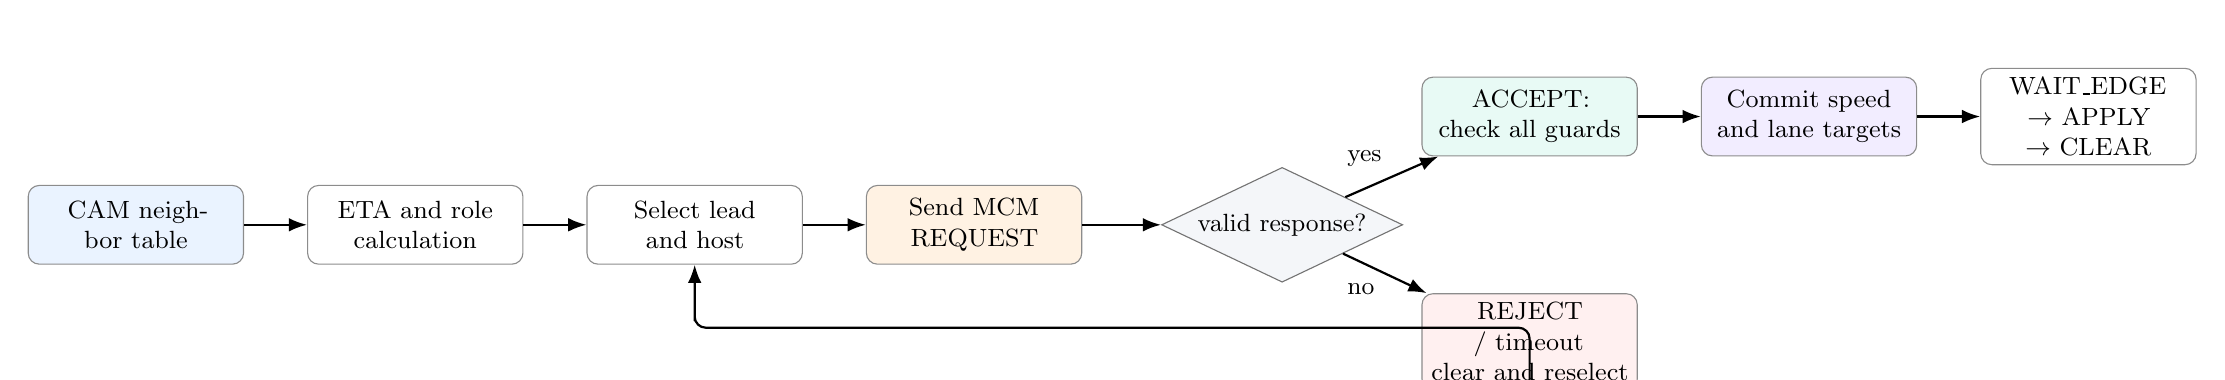
\begin{tikzpicture}[
    >=Latex,
    node distance=7mm and 8mm,
    every node/.style={font=\small, align=center},
    flowbox/.style={draw=black!45, rounded corners, minimum height=10mm, text width=25mm, fill=white},
    decision/.style={draw=black!55, diamond, aspect=2.1, inner sep=1.5pt, fill=lightGray}
]
    \node[flowbox, fill=softBlue] (cam) {CAM neighbor table};
    \node[flowbox, right=of cam] (eta) {ETA and role calculation};
    \node[flowbox, right=of eta] (slot) {Select lead and host};
    \node[flowbox, right=of slot, fill=softOrange] (req) {Send MCM REQUEST};
    \node[decision, right=10mm of req] (resp) {valid response?};
    \node[flowbox, above right=5mm and 10mm of resp, fill=softGreen] (acc) {ACCEPT: check all guards};
    \node[flowbox, below right=5mm and 10mm of resp, fill=softRed] (rej) {REJECT / timeout\\clear and reselect};
    \node[flowbox, right=of acc, fill=softPurple] (cmd) {Commit speed and lane targets};
    \node[flowbox, right=of cmd] (exec) {WAIT\_EDGE $\rightarrow$ APPLY $\rightarrow$ CLEAR};

    \draw[->,thick] (cam) -- (eta);
    \draw[->,thick] (eta) -- (slot);
    \draw[->,thick] (slot) -- (req);
    \draw[->,thick] (req) -- (resp);
    \draw[->,thick] (resp) -- node[above left]{yes} (acc);
    \draw[->,thick] (resp) -- node[below left]{no} (rej);
    \draw[->,thick] (acc) -- (cmd);
    \draw[->,thick] (cmd) -- (exec);
    \draw[->,thick,rounded corners] (rej.south) |- ([yshift=-8mm]slot.south) -| (slot.south);
\end{tikzpicture}}
\caption{End-to-end local decision and execution flow.}
\label{fig:flow}
\end{figure}

\subsection{Host Decision and Reservation}

A main-lane OBU considers only fresh \texttt{REQUEST} messages addressed to itself. If it is already reserving a slot for another merge vehicle, it rejects competing requests. It also rejects a request if it is inside the configured host reject distance or if the temporal gap is too late to create safely.

For merge ETA $\eta_M$, the host computes a target arrival time

\begin{equation}
    \eta_H^\star = \eta_M + h_{\mathrm{safe}} + t_{\mathrm{occupancy}},
\end{equation}

and an approximate required speed

\begin{equation}
    v_H^\star = \frac{d_H}{\max(\eta_H^\star,0.1)}.
\end{equation}

This target is bounded by the host's current speed and by a configurable speed floor. If cooperation is feasible, the host sends \texttt{ACCEPT}, stores the requesting station and maneuver ID, and maintains the reservation while yielding. It periodically retransmits the acceptance and extends the reservation while the ramp vehicle reports \texttt{WAIT\_EDGE}, \texttt{APPLY}, or an active merge. The reservation is released after completion, clear feedback, or a maximum timeout.

\subsection{Finite State Machine}

The OBU uses five states. \texttt{CRUISE} means that no immediate cooperative action is required. \texttt{NEGOTIATING} covers slot selection, request/retry, accepted-but-not-yet-authorized conditions, and waiting for lane availability. \texttt{YIELDING} represents intentional speed reduction by either the merge vehicle or the host. \texttt{MERGING} begins only after physical lane execution is confirmed. \texttt{ABORT} provides a cooldown and cancels unauthorized lane targets.

\begin{figure}[H]
    \centering
    \includegraphics[width=0.98\linewidth]{obu_fsm.png}
    \caption{Finite state machine used by the OBU. Transition labels correspond to the implemented negotiation, execution, recovery, and completion paths.}
    \label{fig:fsm}
\end{figure}

\subsection{Safety Guards}

An MCM acceptance is necessary for a normal host-assisted maneuver, but it is not sufficient. Authorization requires a recent host, valid lead and host temporal clearances, final-lane clearance, merge-zone clearance, projected lead-gap checks, and readiness conditions. The main guards are:

\begin{description}[font=\normalfont\bfseries,leftmargin=0pt,labelindent=0pt,labelsep=0.6em]
    \item[Lead and host temporal gaps.] The merge ETA must remain sufficiently after the lead and before the host.
    \item[Final geometric guard.] Nearby main traffic is checked using Euclidean distance, longitudinal and lateral projections, ETA similarity, and physical clearance.
    \item[Time-to-collision guard.] For a closing rear vehicle, $\mathrm{TTC}=g/(v_r-v_M)$ when $v_r>v_M$. A corresponding front-closing case is evaluated when the merge vehicle is faster. A TTC below the configured threshold blocks authorization.
    \item[Apply and post-clear rear guards.] While the lane command is active, a fast vehicle behind the target lane can force a speed floor. Completion can be delayed until the rear gap or TTC becomes safe.
\end{description}

CAM-based following provides an additional longitudinal layer. For a leader at gap $g$ and closing speed $\Delta v$, the code computes a safe-gap estimate

\begin{equation}
    g_{\mathrm{safe}} = g_{\min} + v_M T + \frac{\max(\Delta v,0)^2}{2a_b},
    \label{eq:safegap}
\end{equation}

where $T$ is the configured headway and $a_b$ is the assumed braking deceleration. When the observed gap is below this value, the OBU reduces its target speed while respecting emergency and post-merge floors.

\subsection{Actuation and Lane Execution Feedback}

The OBU publishes a target speed, optional target lane, and speed mode. The bridge applies speed through \texttt{setSpeed} under full control or \texttt{slowDown} when SUMO's speed mode remains active. Lane execution is stateful:

\begin{table}[H]
\centering
\small
\caption{TraCI lane-command feedback.}
\label{tab:lane_states}
\begin{tabularx}{0.92\linewidth}{L{0.22\linewidth} Y}
\toprule
\textbf{State} & \textbf{Interpretation} \\
\midrule
\texttt{WAIT\_EDGE} & The requested lane index does not exist on the current edge, or the vehicle is on an internal edge where the change cannot be executed. \\
\texttt{APPLY} & The target lane exists and \texttt{traci.vehicle.changeLane()} has been issued or remains active. \\
\texttt{CLEAR} & The vehicle reached the target lane on a non-internal edge; the bridge clears the stored command. \\
\texttt{FAILED} & TraCI raised an exception while applying the lane change. \\
\bottomrule
\end{tabularx}
\end{table}

In the demo, lane index 1 does not exist on ramp edge \texttt{34126779}, whose lane count is 1. The bridge therefore returns \texttt{WAIT\_EDGE}. On main edge \texttt{1331698336}, the lane count becomes 3 and lane index 1 is executable. The OBU then records \texttt{APPLY}, logs \texttt{MERGE\_PHYSICAL\_START}, and enters \texttt{MERGING}. This mechanism prevents a logical acceptance from being incorrectly counted as physical execution.

\subsection{Local Decision Pseudocode}

The principal merge and host loops can be summarized as follows. The pseudocode omits diagnostic logging and recovery branches but preserves the implementation order.

\begin{lstlisting}[style=pseudocode,caption={Simplified merge-vehicle decision loop.},label={lst:merge}]
loop:
    read own sensor state
    update neighbors from CAM and peer status
    estimate own and neighbor ETA to the merge point
    select lead and first non-busy host after own ETA

    if inside request distance and no request exists:
        send REQUEST(host, manoeuvre_id)

    validate only fresh responses from expected host,
    matching target station and manoeuvre_id

    if ACCEPT and temporal/geometric/TTC guards pass:
        authorize and commit the merge
        publish target_speed and target_lane = MERGE_LANE_INDEX

    if lane feedback is WAIT_EDGE:
        remain NEGOTIATING and preserve a safe rolling speed
    if feedback is APPLY or CLEAR:
        mark physical start and enter MERGING
    if target lane reached and rear guard is safe:
        mark COMPLETED and return to CRUISE
\end{lstlisting}

\begin{lstlisting}[style=pseudocode,caption={Simplified host-vehicle decision loop.},label={lst:host}]
on addressed MCM REQUEST:
    discard stale request
    if another reservation is active:
        send REJECT(BUSY)
    else if too close to the merge or gap is too late:
        send REJECT
    else:
        calculate a bounded target speed
        store reservation(requester, manoeuvre_id)
        send ACCEPT
        yield if required

while reservation is active:
    periodically retransmit ACCEPT
    hold the cooperative speed target
    extend during WAIT_EDGE/APPLY/MERGING
    release after completion, clear, or maximum timeout
\end{lstlisting}

\subsection{Regression Validation}

The repository includes repeated headless runs for the denser scenario. \path{scripts/validate_dense_final.sh} checks for tracebacks, warnings, collision messages, \texttt{LANE\_CMD\_FAILED}, and unintended global hostless bypass. It also enforces the invariant that the number of \texttt{MERGE\_PHYSICAL\_START} and \texttt{MERGING!} events equals the total number of completions. These tests complement the visual \texttt{single-lane} demonstration, although the results section below reports only the supplied representative demo trace.

% -----------------------------------------------------------------------------
% 4. Demo flow
% -----------------------------------------------------------------------------
\section{Flow of the Demonstration}

\subsection{Running the Scenario}

The demonstration is started through the scenario wrapper. The command below builds the images, generates the OBU Compose override, launches SUMO-GUI, and starts all per-vehicle services.

\begin{terminalbox}{Single-lane GUI demonstration}
VANETZA_SCENARIO=single-lane \
SUMO_GUI=true \
STEP_DELAY_S=0.05 \
./scripts/run_vanetza_scenario.sh up
\end{terminalbox}

For a reproducible headless log, the same wrapper can be invoked with \texttt{log}, an explicit end time, and a log file path.

\subsection{Observed End-to-End Sequence}

The stored \path{logs/single_lane_host_guard.log} provides a representative trace of the complete process:

\begin{enumerate}
    \item The five OBUs start, publish CAMs, and populate four-neighbor tables.
    \item At $t=\SI{3.0}{s}$, station 105 initially requests cooperation from station 104.
    \item The slot ordering changes while packets are delayed. The merge vehicle creates maneuver 197 for station 103. Station 103 rejects it because the ETA gap is below the minimum host acceptance threshold (\texttt{LATE\_GAP}).
    \item At $t=\SI{8.2}{s}$, the OBU selects station 104 again and creates maneuver 198. Old accepts for maneuver 196 are ignored because the maneuver ID does not match.
    \item At $t=\SI{11.0}{s}$, an acceptance from station 104 for maneuver 198 is matched. The OBU still waits until all slot and clearance conditions pass.
    \item At $t=\SI{12.4}{s}$, the maneuver becomes authorized and committed. The lane command targets lane index 1.
    \item From approximately $t=\SI{13.1}{s}$, the bridge reports \texttt{WAIT\_EDGE}: the ramp and internal edges contain only one lane.
    \item At $t=\SI{16.0}{s}$, main edge \texttt{1331698336} exposes three lanes. The bridge reports \texttt{APPLY}; at $t=\SI{16.2}{s}$ the OBU logs physical start and enters \texttt{MERGING}.
    \item The apply-time and post-clear rear guards protect the merge vehicle while nearby traffic closes from behind. At $t=\SI{31.7}{s}$, the log records a clean completion and a return to \texttt{CRUISE}.
\end{enumerate}

\subsection{Demo Screenshots}

Figure~\ref{fig:demo_request_accept} shows the SUMO view alongside the decoded MCM data. A request from station 105 to station 104 and an acceptance addressed back to station 105 are visible in the terminal output. The screenshot confirms that the V2X transaction is observable independently of the physical simulation window.

\begin{figure}[H]
    \centering
    \includegraphics[width=0.96\linewidth]{image(2).png}
    \caption{Single-lane demonstration showing an MCM request from the merge vehicle and a corresponding acceptance from the selected host.}
    \label{fig:demo_request_accept}
\end{figure}

Figures~\ref{fig:demo_accept} and~\ref{fig:demo_reject} show both response outcomes used by the protocol. Because MCMs are broadcast, all OBUs can decode the packet, but only the target station and matching maneuver process it as an actionable response.

\begin{figure}[H]
    \centering
    \includegraphics[width=0.92\linewidth]{image.png}
    \caption{Decoded MCM \texttt{ACCEPT} message addressed to the merge vehicle while the SUMO scenario continues.}
    \label{fig:demo_accept}
\end{figure}

\begin{figure}[H]
    \centering
    \includegraphics[width=0.92\linewidth]{image(1).png}
    \caption{Decoded MCM \texttt{REJECT} message. The merge OBU does not force the maneuver; it clears or replaces the pending request and recomputes the slot.}
    \label{fig:demo_reject}
\end{figure}

% -----------------------------------------------------------------------------
% 5. Results
% -----------------------------------------------------------------------------
\section{Results and Discussion}

\subsection{Representative Timeline}

Table~\ref{tab:timeline} condenses the most relevant events from the supplied log. It demonstrates not only a successful merge, but also the robustness mechanisms that precede it: host reselection, rejection handling, maneuver-ID validation, delayed lane availability, and rear-gap protection.

\begin{table}[H]
\centering
\small
\caption{Key events in the representative \texttt{single-lane} trace.}
\label{tab:timeline}
\begin{tabularx}{\linewidth}{C{0.15\linewidth} L{0.27\linewidth} Y}
\toprule
\textbf{Time [s]} & \textbf{Event} & \textbf{Interpretation} \\
\midrule
3.0 & \texttt{REQUEST\_SENT}, maneuver 196 & First cooperation attempt, directed to station 104. \\
6.3--8.0 & \texttt{REJECT}, maneuver 197 & Station 103 rejects the alternative slot because the gap is late and below the minimum acceptance margin. \\
8.2 & \texttt{REQUEST\_SENT}, maneuver 198 & Station 104 is selected again with a new maneuver identifier. \\
11.0 & \texttt{ACCEPT\_MATCHED} & Correct host, target, freshness, and maneuver ID are confirmed. \\
12.4 & \texttt{AUTHORIZED} & MCM acceptance and all authorization guards are simultaneously valid. \\
13.1 & \texttt{WAIT\_EDGE} & Target lane 1 does not yet exist on the current one-lane edge. \\
16.2 & \texttt{PHYSICAL\_START} / \texttt{APPLY} & Lane 1 exists on the main edge; physical execution starts. \\
31.7 & \texttt{MERGE\_COMPLETED}, \texttt{clean=True} & Rear-gap completion guard is released and the OBU returns to \texttt{CRUISE}. \\
\bottomrule
\end{tabularx}
\end{table}

The authorization-to-physical-start delay is approximately \SI{3.8}{s}. This delay is expected and useful: it proves that the FSM does not label an authorized maneuver as physically active while the SUMO edge cannot support the requested lane. The physical-start-to-completion interval is longer because the vehicle traverses the lane-change and internal-edge sequence while rear-gap safeguards remain active.

\subsection{What the Demonstration Validates}

The demonstration validates the intended separation of concerns. The OBU observes CAMs, computes ETAs, selects and changes hosts, filters stale MCM responses, and decides when a maneuver is safe. The host maintains its own reservation and speed target. The TraCI bridge independently determines whether the target lane exists and returns execution state. SUMO then performs the physical motion.

The reject screenshot and \texttt{LATE\_GAP} log show that cooperation is not automatically granted. The later successful acceptance shows that the merge vehicle can recover by recomputing the temporal ordering. The \texttt{WAIT\_EDGE} interval demonstrates safe deferred execution, while the final \texttt{clean=True} completion shows that the semantic completion condition includes rear-gap checks rather than only reaching lane index 1.

\subsection{Limitations}

The prototype remains a simulation-oriented engineering demonstrator. The UDP broadcast path does not reproduce a complete wireless channel model with realistic packet loss, congestion, or security. Several parameters and edge identifiers are tuned to the Aveiro scenario; notably, parts of the completion and recovery logic recognize edge \texttt{1331698336} explicitly. The shared FSM status topic also supplements CAM/MCM communication with coordination metadata, so the current system is not a strict CAM-and-MCM-only deployment.

Finally, this report evaluates one representative \texttt{single-lane} run. The repository's dense-run validator supports regression testing, but a statistical performance study would require repeated experiments with controlled seeds, delay and loss profiles, traffic densities, and metrics such as merge time, minimum gap, TTC distribution, retries, and throughput.

% -----------------------------------------------------------------------------
% 6. Conclusion
% -----------------------------------------------------------------------------
\section{Conclusion and Future Work}

The project demonstrates a complete decentralized V2X lane-merging loop in software. Each vehicle is represented by an independent OBU; CAMs provide local awareness; MCMs provide explicit cooperation; ETA ordering identifies the lead and host; and the FSM coordinates request, yield, authorization, execution, and completion. The TraCI bridge provides a clean boundary between strategy and physics by applying commands to SUMO and returning \texttt{WAIT\_EDGE}, \texttt{APPLY}, and \texttt{CLEAR} feedback.

The \texttt{single-lane} demonstration is particularly valuable because it exercises non-ideal paths. A candidate host rejects an unsafe late gap, stale accepts are ignored, another host is selected, authorization is delayed until all guards pass, and physical execution waits until lane 1 exists. The final clean completion confirms the intended end-to-end behavior.

The most relevant future improvements are to remove remaining map-specific constants, add unit tests for slot selection and message matching, automate CSV/plot extraction from logs, introduce configurable delay and packet-loss models, and compare the cooperative algorithm against a non-V2X baseline. A later hardware-in-the-loop step could replace the simulated local brokers and UDP broadcast with real OBU hardware and radio interfaces while preserving the same MQTT and decision-layer contracts.

% -----------------------------------------------------------------------------
% 7. Resources
% -----------------------------------------------------------------------------
\section{Project Resources}

\textbf{Source repository:} \href{\repositoryURL}{\repositoryURL}

\textbf{Demo scenario:} \texttt{single-lane}

\textbf{Demo video:} \emph{Insert the final public video URL, or the permalink to the video message shared in the course Discord channel, before submission.}

% -----------------------------------------------------------------------------
% References
% -----------------------------------------------------------------------------
\begin{thebibliography}{9}

\bibitem{repo}
B. Marujo and A. Alexandre,
\textit{RSA -- Mind the Gap: Autonomous V2X Lane Merging},
GitHub repository. Available at: \url{https://github.com/BMarujo/RSA}.

\bibitem{sumo}
Eclipse SUMO,
\textit{Simulation of Urban MObility Documentation}.
Available at: \url{https://sumo.dlr.de/docs/}.

\bibitem{traci}
Eclipse SUMO,
\textit{TraCI -- Traffic Control Interface}.
Available at: \url{https://sumo.dlr.de/docs/TraCI.html}.

\bibitem{vanetza}
R. Riebl et al.,
\textit{Vanetza: Open-source implementation of the ETSI C-ITS protocol stack}.
Available at: \url{https://github.com/riebl/vanetza}.

\bibitem{mqtt}
Eclipse Foundation,
\textit{Eclipse Mosquitto: An open source MQTT broker}.
Available at: \url{https://mosquitto.org/}.

\bibitem{docker}
Docker Inc.,
\textit{Docker Compose Documentation}.
Available at: \url{https://docs.docker.com/compose/}.

\end{thebibliography}

\end{document}
